% Swiss CPI inflation forecast -- technical report (working draft)
% Status: draft for the meeting of 4 November 2026. Sections marked
% "To be completed" are placeholders for the final report.
\documentclass[11pt,a4paper]{article}
\usepackage[utf8]{inputenc}
\usepackage[T1]{fontenc}
\usepackage{lmodern}
\usepackage[margin=2.5cm]{geometry}
\usepackage{amsmath,amssymb,booktabs,graphicx,caption,xcolor}
\usepackage[hidelinks]{hyperref}
% Figures: the repo's figures/ folder (report compiled in report/) or a
% figures/ folder next to this file (e.g. on Overleaf)
\graphicspath{{../figures/}{figures/}}
\usepackage{parskip}
\usepackage{listings}
\lstset{language=R, basicstyle=\ttfamily\footnotesize, commentstyle=\color{gray},
  keywordstyle=\color{blue!60!black}, columns=fullflexible, frame=single,
  framerule=0.3pt, rulecolor=\color{gray!50}, xleftmargin=1em, framexleftmargin=1em}
\newcommand{\todo}[1]{\textcolor{orange}{\textit{[#1]}}}

\title{Forecasting Swiss CPI inflation, 2026Q4--2029Q3\\[0.3em]
  \large A bottom-up approach with an error correction model for oil products}
\author{Martin Sinishta \and Yanik Bittel \and Evan Weihs\\[0.3em]
  \small Economic Forecasting for Decision Making, HEC Lausanne -- Prof.\ Mathieu Grob\'ety}
\date{Working draft, 4 November 2026}

\begin{document}
\maketitle

\begin{abstract}
\noindent We forecast Swiss year-on-year CPI inflation for 2026Q4--2029Q3 by splitting headline CPI
into four blocks: oil products, rents, imported goods excluding oil and domestic goods and services
excluding rents. Oil products follow an error correction model driven by Brent and the Swiss franc
against the dollar; the other blocks follow univariate ARIMA models. Inflation is forecast at 0.9\%
in 2026Q4, falling to about 0.45\% from mid-2027. A permanent 50\% rise in Brent adds about
0.4 percentage points for one year. Over 55 recursive forecast origins since 2012, the forecasts are
unbiased and beat a headline ARIMA and a random walk at horizons of two to three years, but they are
not efficient: beyond one year they miss turning points.
\end{abstract}

% ==========================================================================
\section{Introduction}
The head of the SNB's forecasting team is mainly concerned that an oil-price shock feeds into Swiss
inflation. We therefore model headline CPI bottom-up and put the exogenous drivers, Brent and the
CHF/USD exchange rate, in the oil block. Section~\ref{sec:data} describes the data,
Section~\ref{sec:models} the models and their optimal forecasts, Section~\ref{sec:forecast} the
forecast, Section~\ref{sec:evaluation} the out-of-sample evaluation and Section~\ref{sec:limits} the
limitations and next steps.
\todo{To be completed: motivation, SNB price-stability range, related literature (e.g.\ Huwiler and Kaufmann, 2013).}

% ==========================================================================
\section{Data and blocks}\label{sec:data}
Monthly CPI indices and basket weights come from the Federal Statistical Office (BFS), Brent from
FRED and CHF/USD from the SNB. Monthly series are converted to quarterly averages. The estimation
sample is 2000Q1--2026Q3 (107 quarters). For each block we use $y_t = 100\ln(\text{index}_t)$, so
$\Delta y_t$ is quarter-on-quarter inflation in percent and $\pi_t = y_t - y_{t-4}$ is year-on-year
inflation.

The BFS publishes imported and domestic aggregates but not the blocks excluding oil and rents. We
build them within each annual chain link (index relative to the previous December), assuming all oil
products are imported and all rents domestic, and chain the links. Weights before 2016 are recovered
from the CPI identity by least squares; against the published 2016--2026 weights the error is at most
0.04 pp.

\begin{table}[h]
  \centering\small
  \caption{Blocks, 2026 basket weights and models}\label{tab:blocks}
  \begin{tabular}{@{}llll@{}}
    \toprule
    Block & Weight & Model & Drivers \\
    \midrule
    Domestic excl.\ rents & 59.0\% & ARIMA(0,1,0)(1,0,0)$_4$ with drift & -- \\
    Imported excl.\ oil   & 20.1\% & ARIMA(2,1,1)(1,0,0)$_4$ with drift & -- \\
    Rents                 & 18.9\% & ARIMA(1,1,1)(1,0,0)$_4$ with drift & -- \\
    Oil products          &  2.1\% & Error correction model & Brent (USD), CHF/USD, trend \\
    \bottomrule
  \end{tabular}
\end{table}

\textbf{Re-aggregation.} Rebuilding headline CPI from the four blocks, linked at Q4 with each year's
weights, reproduces published y-y inflation within 0.14 pp (maximum, 2009) and 0.02 pp on average
since 2000.
\todo{To be completed: descriptive statistics and figure of the four blocks.}

% ==========================================================================
\section{Models and optimal forecasts}\label{sec:models}
Under quadratic loss the optimal $h$-step forecast is the conditional expectation given the
information at the origin $T = $ 2026Q3: future shocks are set to their expected value of zero and
observed values are kept.

\subsection{Oil products: error correction model}
The long-run relation, estimated by OLS (Engle--Granger first step), is
\begin{equation}
  oil_t = \underset{}{247.58} + \underset{(0.014)}{0.428}\, brent_t + \underset{(0.054)}{0.614}\, usd_t
          + \underset{(0.027)}{0.415}\, t + ect_t ,
\end{equation}
where $brent$ is $100\ln$ Brent in USD and $usd$ is $100\ln$ CHF per USD. A 10\% rise in Brent raises
oil-product prices by about 4.3\% in the long run; the elasticity is below one because taxes and
margins are fixed per litre. The short-run dynamics (one lag, chosen by BIC) are
\begin{equation}
  \begin{split}
  \Delta oil_t = {}& \underset{(0.27)}{0.398} \underset{(0.091)}{-\,0.394}\, ect_{t-1}
    + \underset{(0.017)}{0.309}\,\Delta brent_t + \underset{(0.078)}{0.539}\,\Delta usd_t \\
    &+ \underset{(0.077)}{0.017}\,\Delta oil_{t-1} + \underset{(0.037)}{0.095}\,\Delta brent_{t-1}
    \underset{(0.090)}{-\,0.012}\,\Delta usd_{t-1} + \varepsilon_t .
  \end{split}
\end{equation}
About 39\% of a gap to equilibrium closes each quarter. All three variables are I(1) (ADF with trend).
Engle--Granger finds cointegration ($-5.30 < -4.10$ at 5\%); the Johansen trace test does not reject
$r=0$ ($37.98 < 42.44$), but its first cointegrating vector ($0.44$, $0.67$, $0.44$) is close to the
Engle--Granger estimates. Equal Brent and USD elasticities are rejected ($F = 16.7$, $p = 0.0001$).

\textbf{Optimal forecast.} The three equations are iterated forward for $h = 1,\dots,12$:
\begin{align}
  \widehat{\Delta oil}_{T+h} &= c + \alpha\,\widehat{ect}_{T+h-1} + b_0\widehat{\Delta brent}_{T+h}
     + g_0\widehat{\Delta usd}_{T+h} \notag \\
     &\quad + a_1\widehat{\Delta oil}_{T+h-1}
     + b_1\widehat{\Delta brent}_{T+h-1} + g_1\widehat{\Delta usd}_{T+h-1}, \\
  \widehat{oil}_{T+h} &= \widehat{oil}_{T+h-1} + \widehat{\Delta oil}_{T+h}, \\
  \widehat{ect}_{T+h} &= \widehat{oil}_{T+h} - \beta_0 - \beta_1\widehat{brent}_{T+h}
     - \beta_2\widehat{usd}_{T+h} - \delta\,(T+h).
\end{align}
Because Brent and CHF/USD enter contemporaneously, the forecast is conditional on their paths. We
use random walks, so their future changes are zero. Oil inflation then converges to the trend
$\delta = 0.415$ per quarter (about 1.7\% a year), with $ect$ settling at
$(\delta(1-a_1)-c)/\alpha \approx -0.03$.

\subsection{Rents, imported and domestic goods: ARIMA with drift}
Each block follows
\begin{equation}
  \phi(L)\,\Phi(L^4)\,(\Delta y_t - \mu) = \theta(L)\,\varepsilon_t ,
\end{equation}
with drift $\mu$, the mean q-q inflation rate.

\begin{table}[h]
  \centering\small
  \caption{ARIMA estimates, 2000Q1--2026Q3 (standard errors in brackets)}\label{tab:arima}
  \begin{tabular}{@{}lccc@{}}
    \toprule
    & Rents & Imported excl.\ oil & Domestic excl.\ rents \\
    & (1,1,1)(1,0,0)$_4$ & (2,1,1)(1,0,0)$_4$ & (0,1,0)(1,0,0)$_4$ \\
    \midrule
    $\phi_1$   & 0.329 (0.138) & $-0.701$ (0.111) & \\
    $\phi_2$   &               & 0.273 (0.105)    & \\
    $\theta_1$ & 0.529 (0.140) & 0.736 (0.079)    & \\
    $\Phi_1$   & 0.272 (0.101) & 0.514 (0.093)    & 0.725 (0.066) \\
    $\mu$      & 0.357 (0.058) & $-0.140$ (0.167) & 0.149 (0.083) \\
    \midrule
    Ljung--Box $p$ (8 lags) & 0.74 & 0.64 & 0.11 \\
    BIC        & $-21.0$ & 261.3 & 30.0 \\
    \bottomrule
  \end{tabular}
\end{table}

\textbf{Optimal forecast.} Write $a(L) = \phi(L)\Phi(L^4) = 1 - \sum_{i=1}^{P} a_i L^i$ and
$x_t = \Delta y_t - \mu$. Then
\begin{gather}
  \hat x_{T+h} = \sum_{i=1}^{P} a_i\, \hat x_{T+h-i} + \theta_1 \hat\varepsilon_T\, \mathbb{1}[h=1], \\
  \hat y_{T+h} = y_T + \sum_{j=1}^{h}\left(\mu + \hat x_{T+j}\right),
  \qquad
  \hat\pi_{T+h} = \hat y_{T+h} - \hat y_{T+h-4},
\end{gather}
where $\hat x_{T+h-i} = x_{T+h-i}$ for dates up to $T$. As $\hat x$ dies out, $\hat\pi$ converges to
$4\mu$. With $\Delta y_t - \mu = \psi(L)\varepsilon_t$ and cumulated weights
$\Psi_k = \sum_{i=0}^{k}\psi_i$ ($\Psi_k = 0$ for $k<0$), the y-y forecast error variance is
\begin{equation}
  \operatorname{Var}(\pi_{T+h} - \hat\pi_{T+h}) = \sigma^2 \sum_{k=0}^{h-1}\left(\Psi_k - \Psi_{k-4}\right)^2 .
\end{equation}
Our coded recursion reproduces R's \texttt{predict()} to $10^{-13}$. In the imported model the AR
inverse root $-0.98$ nearly cancels the MA root $-0.74$, a sign of over-parameterisation.

\subsection{Aggregation and density}
Block forecasts are converted to index levels and aggregated with the 2026 weights, linked at Q4:
$P^{CPI}_t = P^{CPI}_{Q4,t-1}\sum_i w_i P^i_t / P^i_{Q4,t-1}$. The density forecast uses 5,000
simulated paths; in each future quarter we draw one past quarter and take, from that quarter, the
residuals of all four models and the changes in Brent and CHF/USD, which keeps their correlation.
Parameter uncertainty is not included.

% ==========================================================================
\section{Forecast}\label{sec:forecast}
\begin{figure}[h]
  \centering
  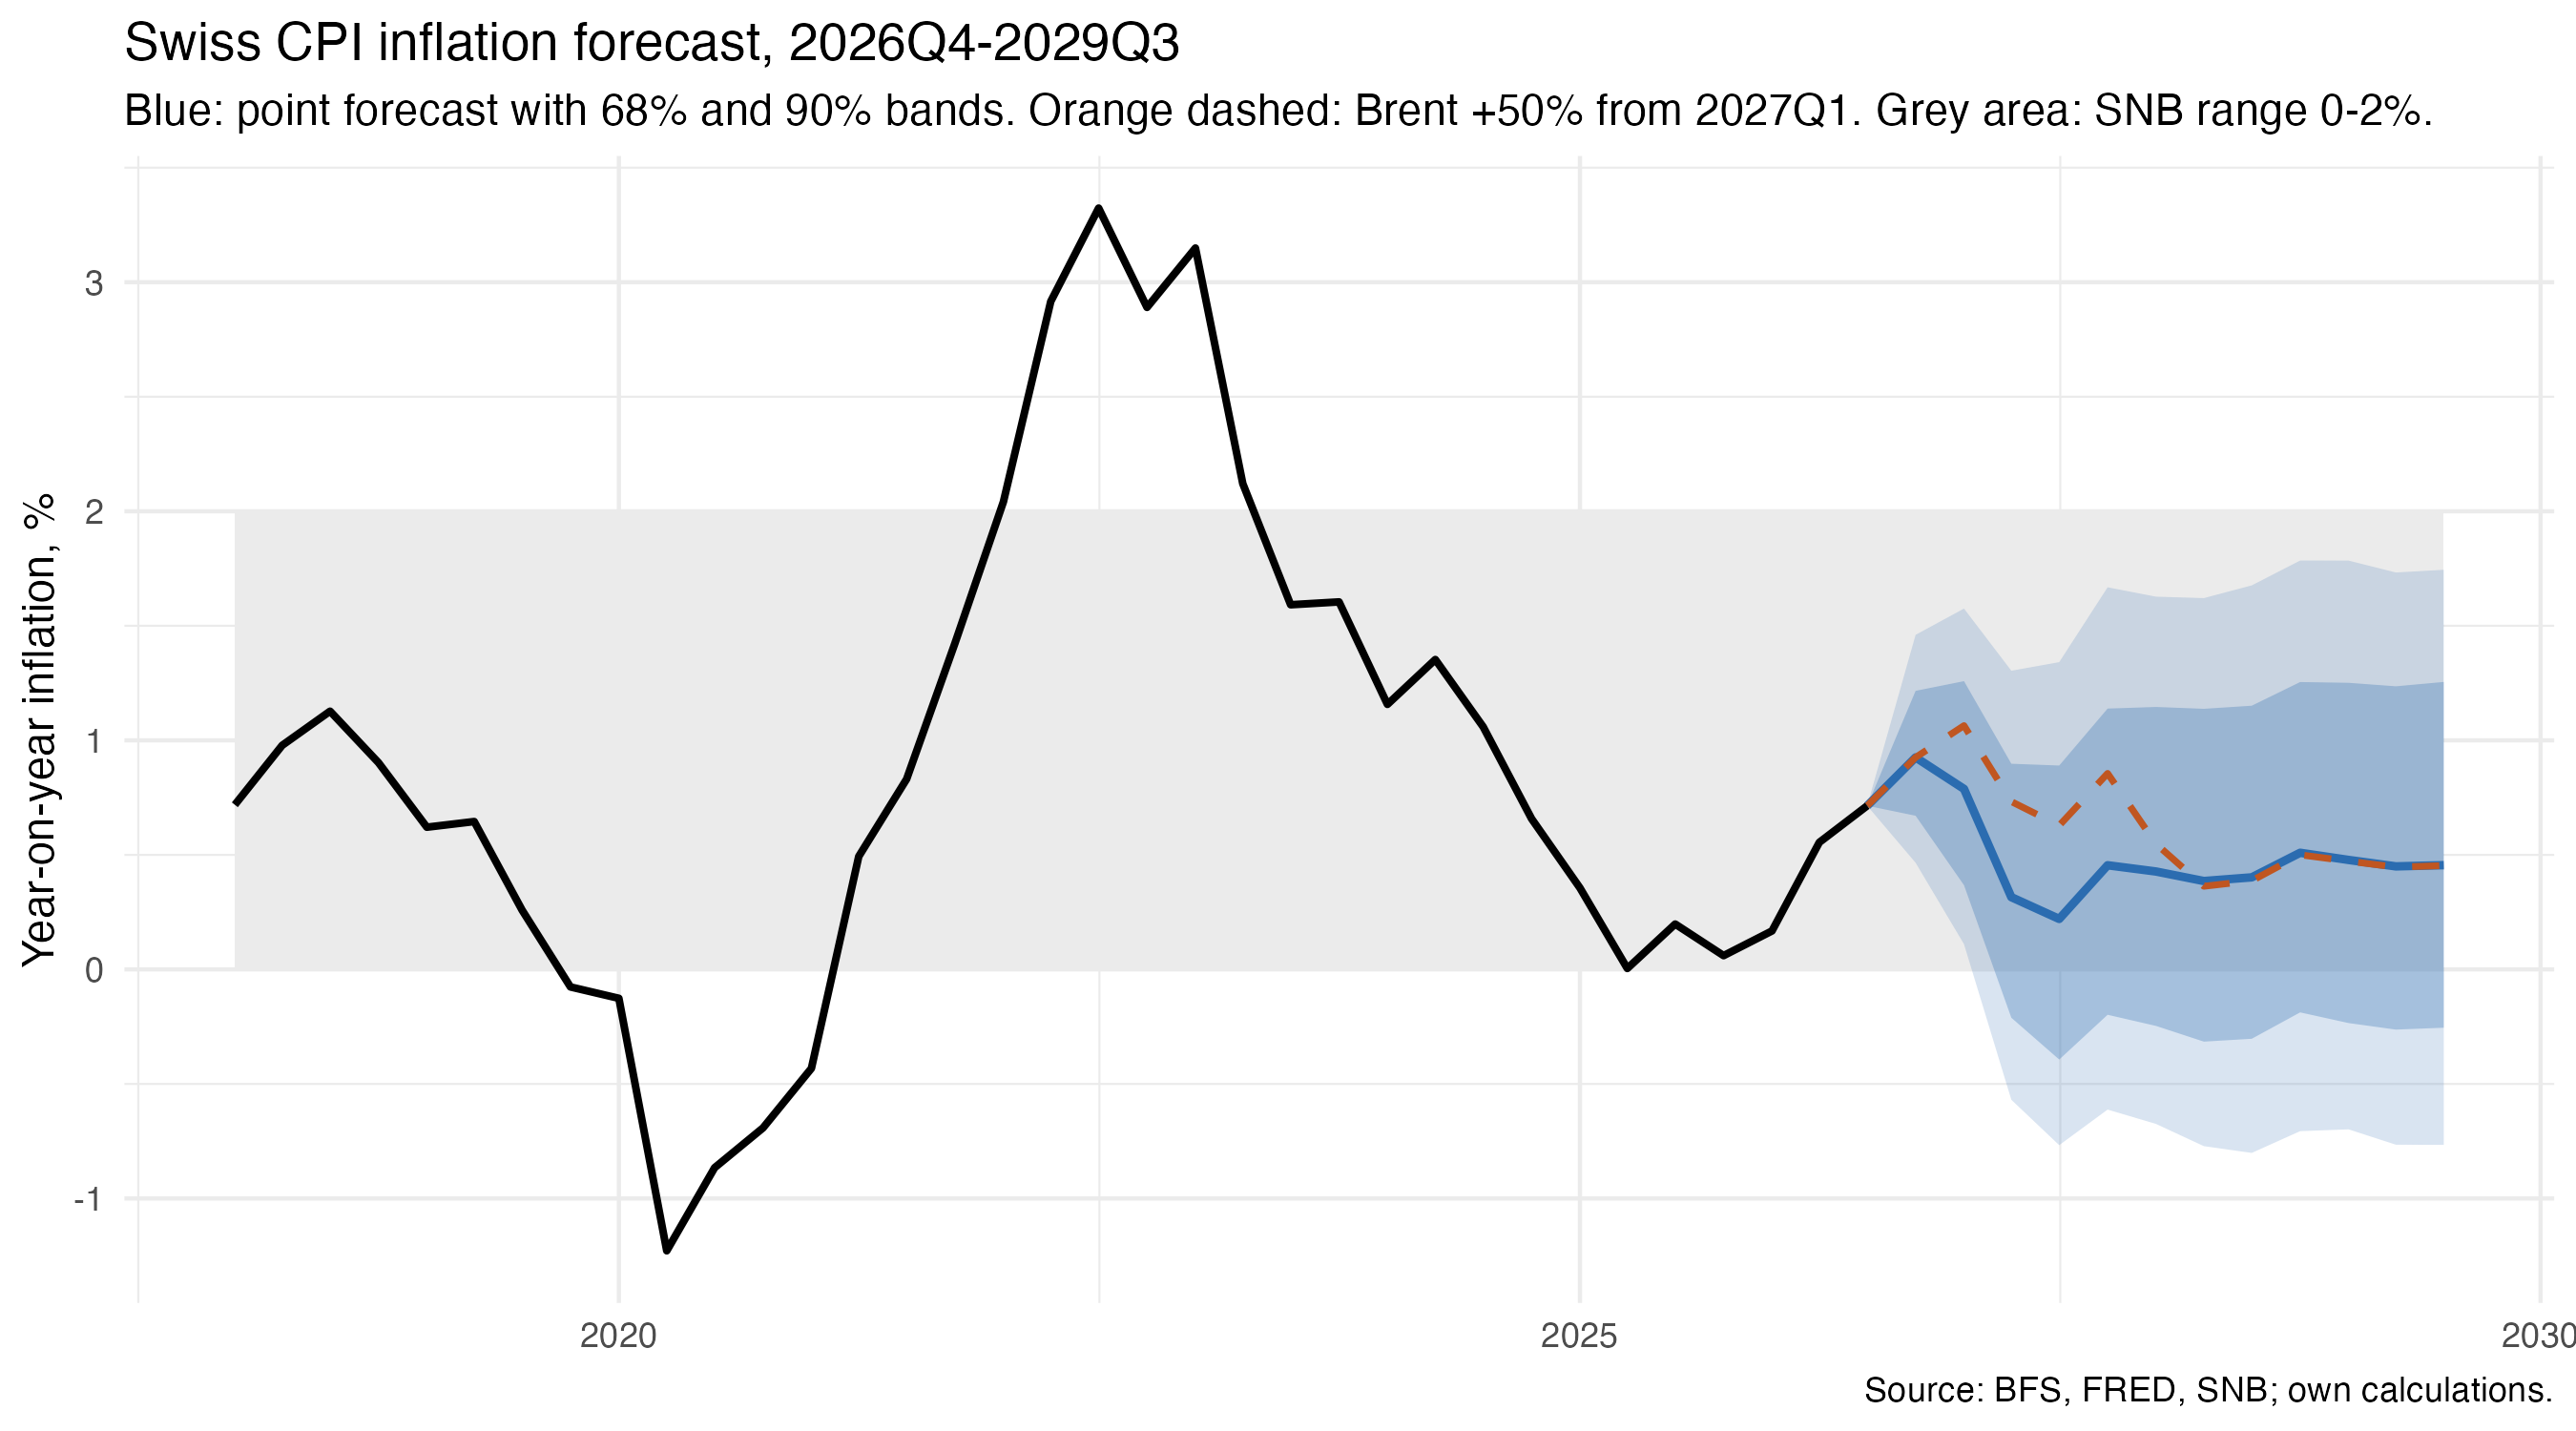
\includegraphics[width=0.85\textwidth]{fan_chart_headline}
  \caption{Headline CPI inflation forecast with 68\% and 90\% bands, and the Brent +50\% scenario}
  \label{fig:fan}
\end{figure}

Headline inflation is forecast at 0.93\% in 2026Q4, a result of the 2026 oil spike (Brent rose from
\$64 in 2025Q4 to \$103 in 2026Q2). As the spike drops out of the y-y rate and oil products return
towards equilibrium, inflation falls to 0.22\% in 2027Q3 and then settles around 0.45\%
(Figure~\ref{fig:fan}). In the long run, rents contribute $+0.27$ pp, domestic goods $+0.28$ pp,
imported goods $-0.13$ pp and oil products $+0.03$ pp. A permanent 50\% rise in Brent from 2027Q1
adds about 0.4 pp for four quarters; it raises the price level permanently but y-y inflation only
for one year.

% ==========================================================================
\section{Out-of-sample evaluation}\label{sec:evaluation}
We produce recursive (expanding-window) forecasts from 55 origins, 2012Q4--2026Q2, for $h = 1,\dots,12$,
re-estimating all models at each origin (Figure~\ref{fig:spaghetti}). Tests follow the lecture
(Section 3.1), with Newey--West standard errors using $h-1$ lags.

\begin{figure}[h]
  \centering
  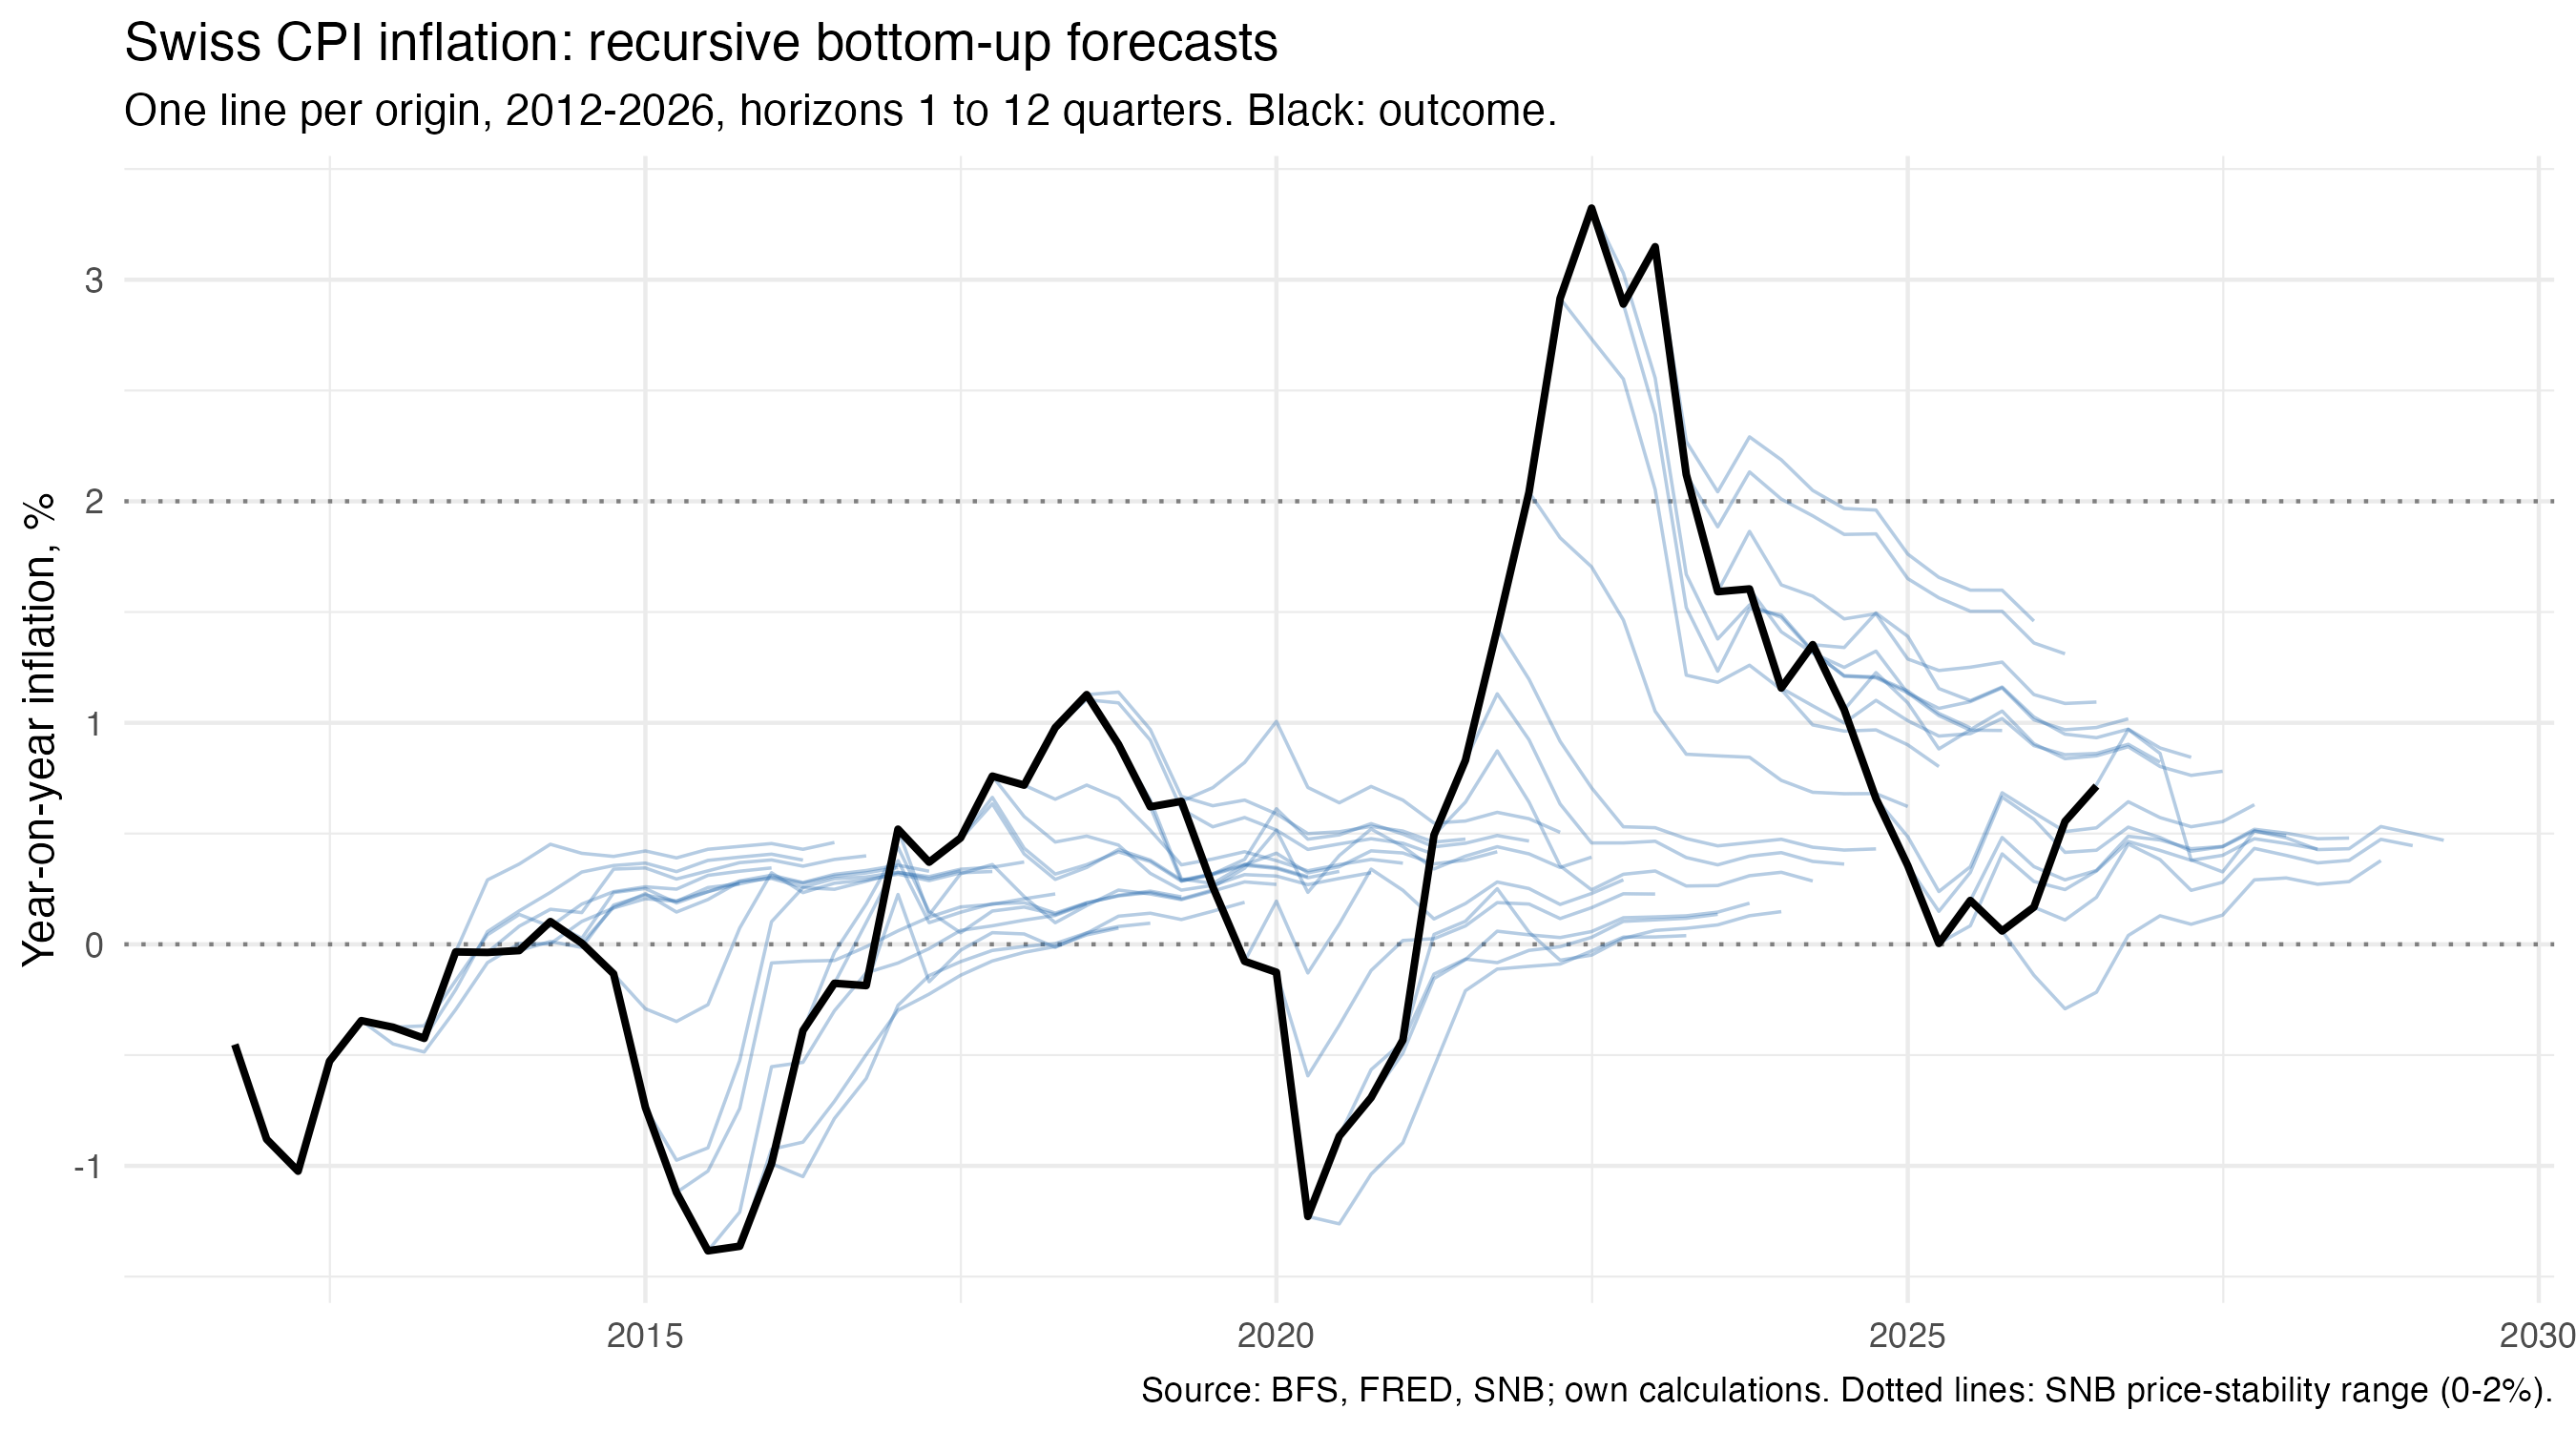
\includegraphics[width=0.85\textwidth]{spaghetti_headline}
  \caption{Recursive bottom-up forecasts against the outcome}
  \label{fig:spaghetti}
\end{figure}

\begin{table}[h]
  \centering\small
  \caption{Absolute standards ($p$-values unless stated)}\label{tab:absolute}
  \begin{tabular}{@{}lcccc@{}}
    \toprule
    & $h=1$ & $h=4$ & $h=8$ & $h=12$ \\
    \midrule
    Mean error (pp) & 0.02 & 0.04 & 0.08 & 0.25 \\
    RMSE (pp) & 0.36 & 1.06 & 1.29 & 1.20 \\
    Unbiasedness, $H_0: \tau = 0$ & 0.71 & 0.90 & 0.84 & 0.50 \\
    Mincer--Zarnowitz, $H_0: \alpha = 0, \beta = 1$ & 0.65 & 0.36 & 0.006 & 0.000 \\
    \quad $\hat\beta$ & 1.06 & 0.64 & $-0.54$ & $-0.53$ \\
    Strong efficiency, $H_0: \beta = 0$ on $\Omega_t$ & 0.013 & 0.038 & 0.005 & 0.000 \\
    Weak efficiency, errors at most MA($h-1$) & 0.015 & 0.001 & 0.001 & 0.24 \\
    \bottomrule
  \end{tabular}
\end{table}

\begin{table}[h]
  \centering\small
  \caption{Relative standards: MSFE ratio, model over benchmark (Diebold--Mariano $p$, HLN correction)}\label{tab:relative}
  \begin{tabular}{@{}lcccc@{}}
    \toprule
    Benchmark & $h=1$ & $h=4$ & $h=8$ & $h=12$ \\
    \midrule
    ARIMA on headline CPI & 0.99 (0.97) & 1.04 (0.80) & 0.80 (0.04) & 0.75 (0.04) \\
    Random walk on y-y inflation & 0.78 (0.29) & 0.84 (0.39) & 0.56 (0.02) & 0.46 (0.07) \\
    Sample mean & 0.11 (0.00) & 0.85 (0.31) & 1.17 (0.35) & 1.11 (0.47) \\
    \bottomrule
  \end{tabular}
\end{table}

The forecasts are unbiased at all horizons (Table~\ref{tab:absolute}). The bottom-up model beats the
headline ARIMA by 20--25\% in MSFE at $h = 8$--12 and the random walk at all horizons
(Table~\ref{tab:relative}), so the disaggregation adds value at medium horizons. Beyond one year,
however, Mincer--Zarnowitz and both efficiency tests reject and the model does no better than the
sample mean: it extrapolates the current situation and misses turning points, such as the 2022 surge
and the 2024--25 decline. MAFE ratios give the same ranking.
\todo{To be completed: density evaluation (coverage, PIT), error variance by horizon.}

% ==========================================================================
\section{Limitations and next steps}\label{sec:limits}
\begin{itemize}
  \item \textbf{Seasonality.} The ARIMA models contain seasonal AR terms. Next: seasonality plots by
        quarter, X-13 adjustment where seasonal, plain ARIMA.
  \item \textbf{Persistence beyond one year.} Next: test deterministic against stochastic trends for
        domestic goods (ADF with trend).
  \item \textbf{Imported block.} The negative drift ($-0.14$, not significant) lowers headline
        inflation by 0.13 pp over the whole horizon, and the AR and MA roots nearly cancel. Next: drop
        the drift or add a 2009--2016 dummy; estimate ARIMA(1,1,0) or (0,1,1).
  \item \textbf{Density bands.} The 90\% half-width at $h=8$ is 1.24 pp, against about 2.1 pp implied
        by the out-of-sample RMSE. Next: check coverage and calibrate on out-of-sample errors.
  \item \textbf{Outliers.} COVID and 2022: additive outliers where a residual exceeds three times the
        interquartile range.
\end{itemize}

% ==========================================================================
\section*{Questions for the meeting of 4 November}
\begin{enumerate}
  \item Is X-13 seasonal adjustment followed by a plain ARIMA acceptable for the non-oil blocks?
  \item Engle--Granger finds cointegration and Johansen does not: is Engle--Granger enough to keep the ECM?
  \item Can we extrapolate the ECM's linear trend for 12 quarters, or should CO$_2$-levy dummies replace it?
  \item Brent and CHF/USD: random walk plus a shock scenario, or the futures curve?
  \item Imported block: drop the drift, add a 2009--2016 dummy, or start the sample later?
  \item Are the least-squares weights before 2016 (maximum error 0.04 pp) acceptable?
\end{enumerate}

% ==========================================================================
\appendix
\section{Code and reproducibility}\label{app:code}
All results come from one R project. Running \texttt{source("main.R")} reproduces every table and
figure in about 30 seconds. Parameters (sample start, horizon, model orders, first evaluation
origin, number of simulations, scenario) are set once at the top of \texttt{main.R}. Raw data are
downloaded through APIs (BFS, FRED, SNB), never edited by hand, and all paths are relative
(\texttt{here()}).

\begin{verbatim}
Forecasting/
|-- main.R                     parameters + runs everything in order
|-- R/functions.R              download helpers
|-- R/models.R                 model, forecast, aggregation and test functions
|-- Scripts/01_load_data.R     raw data from the APIs into RAW_DATA/
|-- Scripts/02_dta_cleaning.qmd  cleaning, block indices, weights, quarterly data
|-- Scripts/04_model_estimation.R  estimates, diagnostics, cointegration, checks
|-- Scripts/05_forecasting.R   point and density forecast, scenario, fan chart
|-- Scripts/06_evaluation.R    recursive forecasts, evaluation tables, charts
|-- DTA_CLEAN/  output/  figures/  report/
\end{verbatim}

Estimation uses transparent functions only (\texttt{stats::arima} by maximum likelihood,
\texttt{lm}, \texttt{urca}); no automatic model selection. The forecasts are coded by hand from the
derivations in Section~\ref{sec:models}, so each equation has a matching function
(Table~\ref{tab:functions}).

\begin{table}[h]
  \centering\small
  \caption{Main functions in \texttt{R/models.R}}\label{tab:functions}
  \begin{tabular}{@{}lp{0.52\textwidth}l@{}}
    \toprule
    Function & What it does & Implements \\
    \midrule
    \texttt{fit\_arima()} & ARIMA$(p,1,q)(P,0,Q)_4$ with drift, by ML & eq.~(6) \\
    \texttt{arima\_polys()} & Multiplies out $a(L)=\phi(L)\Phi(L^4)$ and the MA side & eq.~(7) \\
    \texttt{arima\_paths()} & Iterates the ARIMA forward, back to log levels; zero shocks give the point forecast, drawn shocks give simulated paths & eq.~(7)--(8) \\
    \texttt{fit\_ecm()} & Engle--Granger two steps: long-run OLS, then short-run OLS with $ect_{t-1}$ & eq.~(1)--(2) \\
    \texttt{ecm\_paths()} & Iterates the three ECM equations forward, given driver paths & eq.~(3)--(5) \\
    \texttt{aggregate\_headline()} & Rebuilds headline y-y inflation from block levels, linked at Q4 & Section~3.3 \\
    \texttt{forecast\_point()} & Fits all four blocks at one origin and returns the headline forecast & -- \\
    \texttt{wald\_hac()} & Wald test with Newey--West covariance ($h-1$ lags): MZ, unbiasedness, strong efficiency & Table~\ref{tab:absolute} \\
    \texttt{weak\_efficiency\_p()} & Ljung--Box on the residuals of an MA$(h-1)$ fitted to the errors & Table~\ref{tab:absolute} \\
    \texttt{dm\_test()} & Diebold--Mariano with the Harvey--Leybourne--Newbold correction & Table~\ref{tab:relative} \\
    \bottomrule
  \end{tabular}
\end{table}

Check of the derivation: with zero shocks, \texttt{arima\_paths()} returns the same forecasts as R's
Kalman-filter \texttt{predict()}, with a maximum difference of $10^{-13}$ for all three blocks. The core
of the recursion, steps 2 and 3 of eq.~(7)--(8):

\begin{lstlisting}
for (j in 1:h) {
  t  <- n_x + j
  ar <- colSums(pl$a * X[t - seq_len(P), , drop = FALSE])  # sum of a_i * x_{T+h-i}
  ma <- colSums(pl$m * E[t - seq_len(Q), , drop = FALSE])  # MA terms: eps_T only at h = 1
  X[t, ] <- ar + E[t, ] + ma                                # future shocks E = 0 (point)
}
dy <- X[n_x + 1:h, , drop = FALSE] + pl$mu                  # back to q-q inflation
y[length(y)] + matrix(apply(dy, 2, cumsum), h, N)           # cumulate to log levels
\end{lstlisting}

\end{document}
